\section{ТРЕУГОЛЬНИКИ}

\textbf{1695.}  $180-(36+73)=71.$  \newline \null \hfill  Ответ: 71.

\textbf{1695-1697.}  - аналогичные задачи. 

\textbf{1698.} $90-57=33.$ \newline \null \hfill Ответ: 33. 

\textbf{1699-1700.}  - аналогичные задачи. 

\textbf{1701.} $\frac{64}{2} = 32.$ \newline \null \hfill Ответ: 32.

\textbf{1702-1703.} аналогичные задачи.

\textbf{1704.} $AM = \frac{AC}{2} = 29$. \newline \null \hfill Ответ: 29.

\textbf{1705-1706.} аналогичные задачи.

\textbf{1707.} $MN = \frac{AC}{2} = 17.$ \newline \null \hfill Ответ: 17.

\textbf{1708-1709.} аналогичные задачи.

\textbf{1710.} $S = \frac{18 \cdot 7}{2} = 63$. \newline \null \hfill Ответ: 63.

\textbf{1711-1712.} аналогичные задачи.

\textbf{1713.} $S = \frac{ah}{2} = \frac{18 \cdot 17}{2} = 153$. \newline \null \hfill Ответ: 153.

\textbf{1714-1715.} аналогичные задачи.

\textbf{1716.} Катет $ВС$, лежащий против угла $А$, равного $30^\circ$, равен половине гипотенузы $АВ$, т.е. равен 20. 
\newline \null \hspace*{\fill} Ответ: 20.

\textbf{1717.} аналогичная задача.

\clearpage

\textbf{1718.} 

{\centering 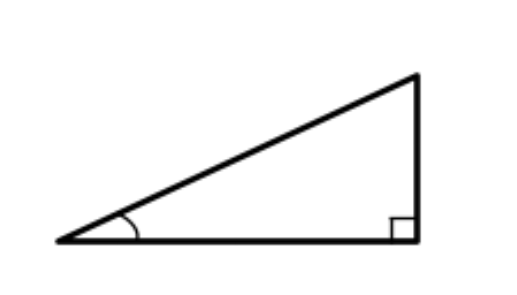
\includegraphics[width=0.4\linewidth]{Geometry/Content/1.png}
\[
\frac{AC}{AB} = \cos{A} = \frac{\sqrt{3}}{2}, \; AB = \frac{AC}{\sqrt{3} / 2} = \frac{34 \sqrt{3}}{\sqrt{3} / 2} = 68.
\]
\newline \null \hspace*{\fill} Ответ: 68.
}

Задачи \textbf{1719-1727} решаются аналогично, т.е. с использованием понятий синуса, косинуса угла и их значений для углов $30^\circ$ и $60^\circ$.

\textbf{1728.} По теореме Пифагора $c = \sqrt{a^2 + b^2} = \sqrt{9^2 + 40^2} = \linebreak = \sqrt{1681} = 41$ \newline \null \hspace*{\fill} Ответ: 41.

Аналогично, т.е. на основании теоремы Пифагора,  решаются задачи \textbf{1729-1735.}

\textbf{1736.}


{\centering 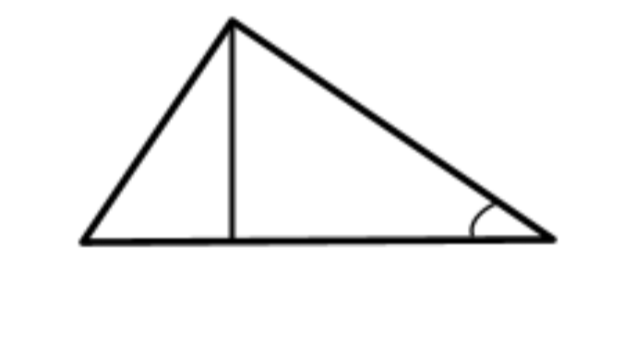
\includegraphics[width=0.4\linewidth]{Geometry/Content/2.png}
	
}

Возможны два решения.

1. Т.к $BC \cdot AC = AB \cdot CH$ (как удвоенные площади треугольника), то 
\begin{eqnarray*}
CH = \frac{BC \cdot AC}{AB} = \frac{AB \sin{30^\circ}\cdot AB \cos{30^\circ}}{AB} = \\=AB \sin{30^\circ}\cos{30^\circ} = 36\sqrt{3}\cdot\frac{1}{2}\cdot\frac{\sqrt{3}}{2} = 27.
\end{eqnarray*}
2. Из $\Delta ABC:$ $AC = AB\cos{30^\circ} = 36\sqrt{3}\cdot \frac{\sqrt{3}}{2} = 54.$

Из $\Delta CAH:$ $CH = \frac{AC}{2} = 27.$ \newline \null \hspace*{\fill} Ответ: 27.

\clearpage 

Аналогичные соображения позволяют решить задачи  \textbf{1739-1743}.

\textbf{1744.}

{\centering 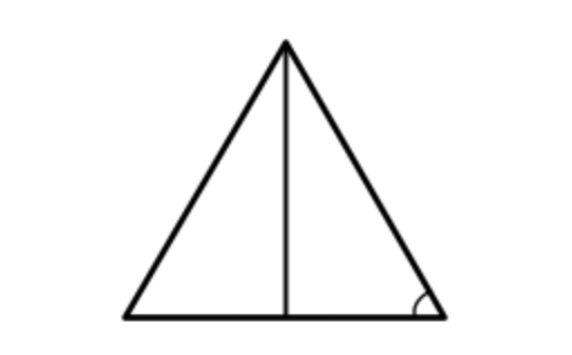
\includegraphics[width=0.4\linewidth]{Geometry/Content/3.png}
	
}

Т.к. $\Delta ABC$ - равносторонний, его углы равны по $60^\circ$. Поскольку $CH$ - высота, то $\Delta CAH$ - прямоугольный. Тогда 
\[
CH = AC \sin{60^\circ} = 2\sqrt{3}\cdot\frac{\sqrt{3}}{2} = 3.
\] \null \hspace*{\fill} Ответ: 3.

Задачи \textbf{1745-1749} решаются аналогично.

\textbf{1750.}

{\centering 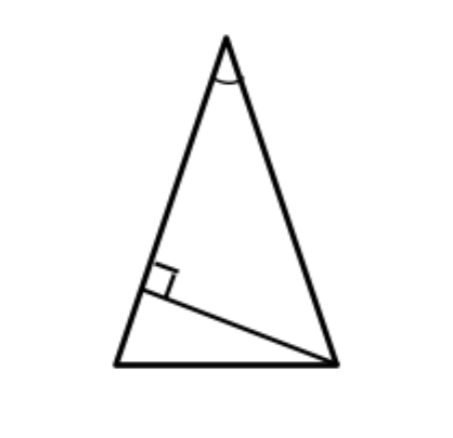
\includegraphics[width=0.4\linewidth]{Geometry/Content/4.png}
	
}

$\Delta CAH$ -  прямоугольный треугольник с острым углом $30^\circ$. Тогда
\[
CH = \frac{AC}{2} = 11
\].\null \hspace*{\fill} Ответ: 11.

Аналогично решаются задачи \textbf{1751-1755}.

\textbf{1756.} Если $\alpha$ и $\beta$ - острые углы прямоугольного треугольника ($\alpha > \beta$), то:

{\centering $
\begin{cases}
	\alpha + \beta = 90 \\
	\alpha - \beta = 79
\end{cases}
$, откуда $2\alpha = 169$, $\alpha = 84,5^\circ$ \newline \null \hspace*{\fill} Ответ: 84,5.

}

\textbf{1757-1759.} анлогичные задачи.

\textbf{1760.}

{\centering 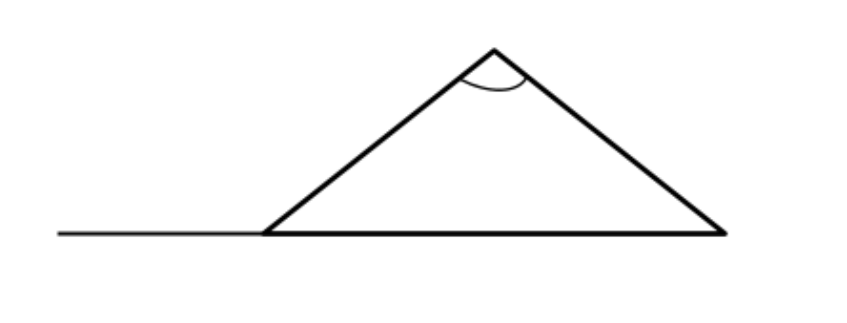
\includegraphics[width=0.6\linewidth]{Geometry/Content/5.png}

}

Т.к. $\Delta ABC$ - равнобедренный, то $\angle CBA = \angle CAB = \frac{180^\circ - 116^\circ}{2} = \linebreak =32^\circ$, а $\angle CBD = 180^\circ - \angle CBA = 148^\circ.$ \newline \null \hspace*{\fill} Ответ: 148.

Задачи \textbf{1761-1764} - аналогичные.

\textbf{1765.}

{\centering 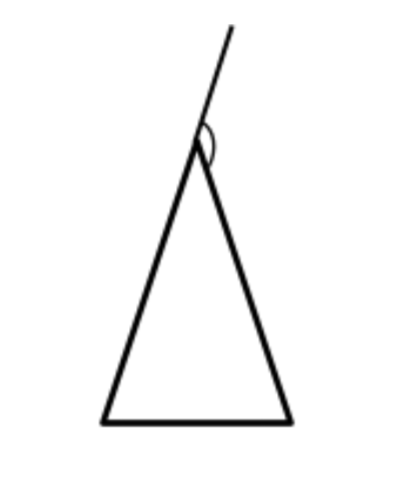
\includegraphics[width=0.3\linewidth]{Geometry/Content/6.png}

}

Т.к. задан внешний угол, то угол при вершине равен $180^\circ - 150^\circ = \linebreak
=30^\circ$.

$\Delta ABC$ - равнобедренный, поэтому $\angle B = \angle A = \frac{180^\circ - 30^\circ}{2} = 75^\circ$.

\null \hspace*{\fill} Ответ: 75.

\textbf{1766, 1767} - аналогичные задачи.

\textbf{1768.} Пусть и $\alpha$ и $\frac{\alpha}{4}$ - углы треугольника, не смежные с внешним углом $15^\circ$. Поскольку внешний угол треугольника равен сумме углов, не смежных с ним, то

{\centering $\alpha + \frac{\alpha}{4} = 15^\circ$, откуда $\alpha =12^\circ$. \newline \null \hspace*{\fill} Ответ: 12.

}

\textbf{1769-1771} - аналогичные задачи.

\textbf{1772.}  Поскольку задан тупой угол, равный $98^\circ$, то это есть угол при вершине равнобедренного треугольника. Тогда  $98^\circ + 2\alpha = \linebreak= 180^\circ$, где $\alpha$ - угол при основании. Очевидно, 
\[
\alpha = \frac{180^\circ - 98^\circ}{2} = 41^\circ
\].\null \hspace*{\fill} Ответ: 41.

\textbf{1773-1775} - аналогичные задачи.

\textbf{1776.} Пусть $\alpha$ - сумма двух углов треугольника, а $\beta$ - внешний угол, смежный с третьим углом. Тогда $\alpha = \beta$, а по условию задачи $\alpha + \beta = 68^\circ$. Отсюда $\alpha = 34^\circ$, так что  третий угол равен $180^\circ - \alpha = 146^\circ$. \newline \null \hspace*{\fill} Ответ: 146.
 
\textbf{1777-1779} - аналогичные задачи.

\textbf{1780.}

{\centering 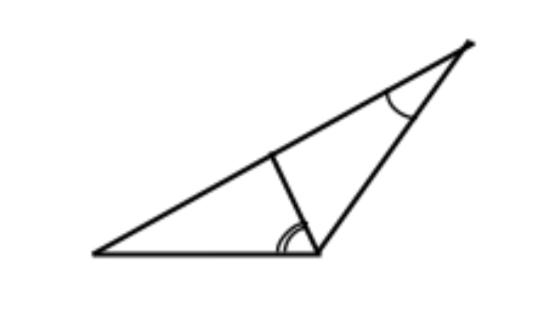
\includegraphics[width=0.5\linewidth]{Geometry/Content/7.png}
	
}

Поскольку $AD$ - биссектриса, то $\angle DAC = \angle DAB = 69^\circ$. Искомый угол $ADB$ является для $\Delta ADC$ внешним углом, смежным с углом $ADC$, поэтому $\angle ADB = \angle C + \angle DAC = 30^\circ + 69^\circ = 99^\circ.$ \newline \null \hspace*{\fill} Ответ: 99.

\textbf{1781-1783.} - аналогичные задачи.

\clearpage 

\textbf{1784.}

{\centering 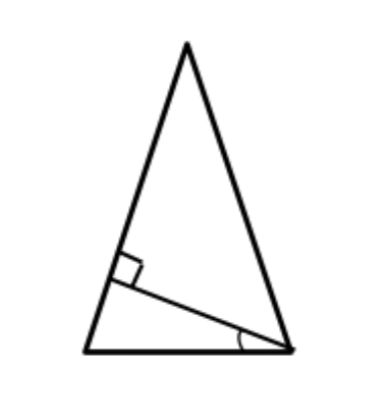
\includegraphics[width=0.4\linewidth]{Geometry/Content/8.png}
	
}

В прямоугольном треугольнике $DAB$ $\angle B = 90^\circ - 19^\circ = 71^\circ$. В равнобедренном треугольнике $ABC$ углы при основании равны, поэтому $\angle C = 180^\circ - 2\cdot 71^\circ = 38^\circ.$ \newline \null \hspace*{\fill} Ответ: 38.

\textbf{1785-1787} - аналогичные задачи.

\textbf{1788.}

{\centering 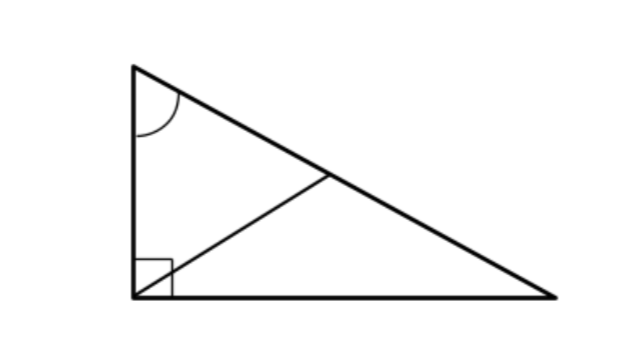
\includegraphics[width=0.5\linewidth]{Geometry/Content/9.png}
	
}

Точка $D$ - середина гипотенузы; она является центром описанной около $\Delta ABC$ окружности. Поэтому $\Delta ACD$ равнобедренный и $\angle ACD = \angle A = 90^\circ - \angle B = 35^\circ.$ 
\newline \null \hspace*{\fill} Ответ: 35

\textbf{1789-1791.} - аналогичные задачи.

\clearpage 

\textbf{1791.}

{\centering 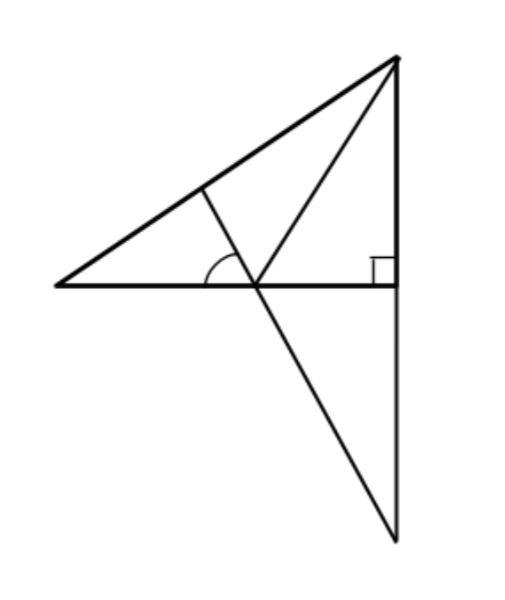
\includegraphics[width=0.4\linewidth]{Geometry/Content/10.png}
	
}

Т.к. $\angle BAD = \angle DAC = 74^\circ$, то $\Delta ABC$ - тупоугольный, поэтому основание высоты $CH$ находится на продолжении стороны $AB$, а точка $O$ пересечения высоты $CH$ и биссектрисы $AD$ находится вне $\Delta ABC$. $\angle BAD = \angle OAH = 74^\circ$  как вертикальные углы. $\Delta AOH$ - прямоугольный, поэтому $\angle AOC = \angle O = 90^\circ - 74^\circ =\linebreak = 16^\circ$. \newline \null \hspace*{\fill} Ответ: 16.

Аналогично решается задача \textbf{1793}.

\textbf{1794.}

{\centering 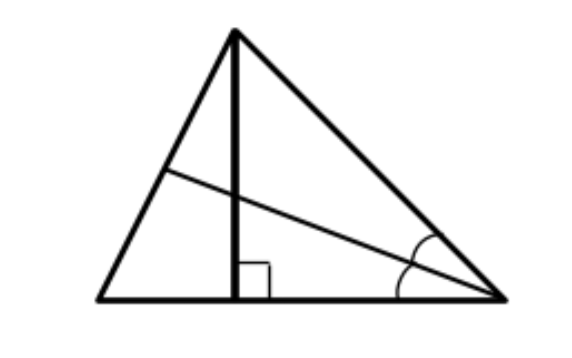
\includegraphics[width=0.4\linewidth]{Geometry/Content/11.png}
	
}

Т.к. $CH \perp AB$, то $\Delta AHO$ - прямоугольный. $\angle AOC$ - внешний угол этого треугольника. Он равен сумме углов $\Delta AHO$, не смежных с ним, т.е
$\angle AOC = 90^\circ + 30^\circ = 120^\circ$. \newline \null \hspace*{\fill} Ответ: 120.

\textbf{1795} - аналогичная задача.

\clearpage 

\textbf{1796.}

{\centering 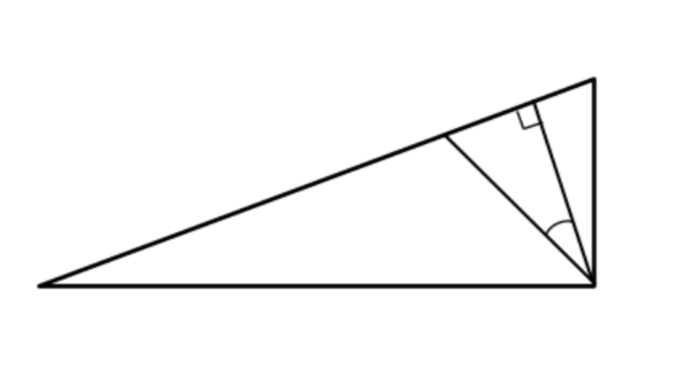
\includegraphics[width=0.5\linewidth]{Geometry/Content/12.png}
	
}

Пусть в $\Delta ABC$ $CD$ и $CH$ - биссектриса и высота, проведенные из вершины $C$ прямого угла, а $\angle A$ - меньший угол треугольника; $\angle DCH = 37^\circ$. Тогда в прямоугольном $\Delta DHC$ $\angle HDC = 90^\circ -\linebreak - 37^\circ = 53^\circ.$

Теперь рассмотрим $\Delta ADC$. В нем $\angle DCA = 45^\circ$, т.к. $CD$ - биссектриса прямого угла. Найденный ранее $\angle HDC$ является для $\Delta ADC$ внешним, так что $\angle A = \angle HDC - \angle DCA  = 53^\circ - 45^\circ = 8^\circ.$ 

\null \hspace*{\fill} Ответ: 8.

\textbf{1797-1799} - аналогичные задачи.

\textbf{1802.}

{\centering 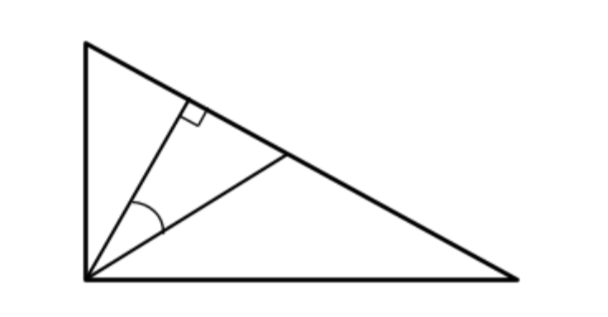
\includegraphics[width=0.5\linewidth]{Geometry/Content/13.png}
	
}

Пусть в $\Delta ABC$ $CD$ и $CH$ - медиана и высота, проведенные из вершины $C$ прямого угла, а $\angle B$ - больший угол треугольника; $\angle DCH = 31^\circ$. Тогда в прямоугольном $\Delta DHC$ $\angle HDC = 90^\circ - \linebreak -31^\circ = 59^\circ$. 

Теперь рассмотрим $\Delta BDC$. Т.к. точка $D$ - середина гипотенузы, то $BD = CD$ (как радиусы описанной окружности). Поэтому $\Delta BDC$ - равнобедренный и $\angle B = \angle BCD = \frac{180^\circ - 59^\circ}{2} = 60,5^\circ$

 \null \hspace*{\fill} Ответ: 60,5.

Аналогичным образом решаются задачи \textbf{1800, 1801}. 

\textbf{1803.}

{\centering 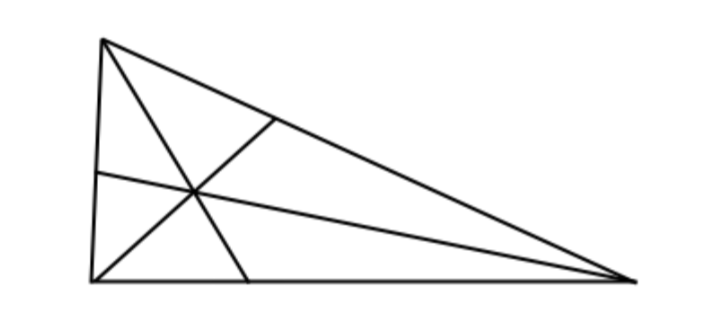
\includegraphics[width=0.5\linewidth]{Geometry/Content/14.png}
	
}
\[
\angle C = 180^\circ - \angle A - \angle B = 180^\circ - 25^\circ - 89^\circ = 66^\circ.
\]
 Рассмотрим $\Delta COA$. В нем $\angle OCA = \frac{\angle C}{2} = 33^\circ$, $\angle OAC = \frac{\angle A}{2} = \linebreak = 12,5^\circ$. В силу того, что искомый $\angle AOF$ для этого треугольника является внешним, получаем:
\[
\angle AOF = \angle OCA + \angle OAC = 45,5^\circ.
\] \null \hspace*{\fill} Ответ: 45,5. 

\textbf{1804-1806} - аналогичные задачи.

\textbf{1807.}

{\centering 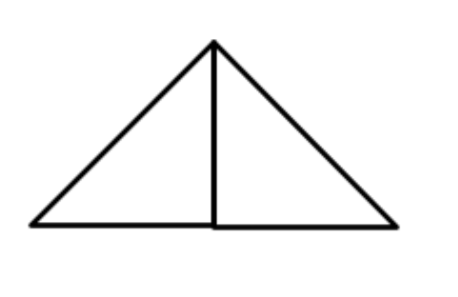
\includegraphics[width=0.4\linewidth]{Geometry/Content/15.png}
	
}

Поскольку в треугольнике $ABC$ два угла равны по $45^\circ$, то треугольник прямоугольный, его высоты пересекаются в вершине прямого угла $C$, т.е. точка $C$ совпадает с точками $O$, $D$, $E$. Поэтому $\angle AOF = 45^\circ$. \newline \null \hspace*{\fill} Ответ: 45.

\textbf{1808.}

{\centering 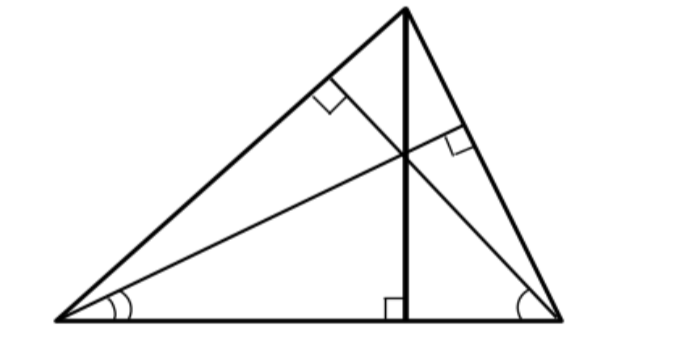
\includegraphics[width=0.4\linewidth]{Geometry/Content/16.png}
	
}

Поскольку сумма углов $A$ и $B$ меньше $90^\circ$, то $\Delta ABC$ - тупоугольный и точка $O$ пересечения его высот находится вне треугольника. Т.к. $CF \perp AB$, то $\Delta CFB$ - прямоугольный и $\angle FCB = \linebreak= 90^\circ - 39^\circ = 51^\circ$.  Аналогично $\Delta ODC$ - также прямоугольный, а $\angle DCO = \angle FCB = 51^\circ$ как вертикальные. Поэтому $\angle AOF = \linebreak=90^\circ - 51^\circ = 39^\circ.$ (Тот же результат следует из подобия треугольников $CFB$ и $ODC$). \newline \null \hspace*{\fill} Ответ: 39.

\textbf{1809, 1810} - аналогичные задачи.

\textbf{1811.}

{\centering 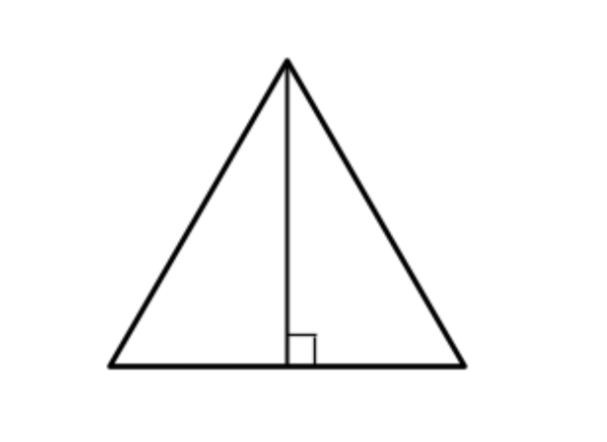
\includegraphics[width=0.5\linewidth]{Geometry/Content/17.png}
	
}

Т.к. $AC=BC$, то $\Delta ABC$ - равнобедренный, его высота $CH$ является медианой: $AH = \frac{AB}{2}=43$ . В прямоугольном $\Delta AHC$ $tgA=\frac{CH}{AH} = \sqrt{3}$, угол $A = 60^\circ$. Таким образом, $\Delta ABC$ - равносторонний, поэтому и угол $C = 60^\circ.$
\newline \null \hspace*{\fill} Ответ: 60.

\textbf{1812-1814} - аналогичные задачи.

\textbf{1815.}  Площадь прямоугольного треугольника $S = \frac{ab}{2}$, где $a$ и \newline $b$ - длины его катетов. Поэтому
\[
b = \frac{2S}{a} = \frac{2 \cdot 69}{23} = 6
\]. \null \hspace*{\fill} Ответ: 6.

\textbf{1816-1818} - аналогичные задачи.

\textbf{1819.} Площадь треугольника $S = \frac{ab\sin{\alpha}}{2}$, где $a$, $b$ и $\alpha$ - длины двух сторон и угол между ними. В нашем случае $a = b = 2$, $\alpha = 150^\circ$, так что
\[
S = \frac{2 \cdot 2 \sin{150^\circ}}{2} = \frac{2 \cdot 2 \cdot \frac{1}{2}}{2} = 1
\].\null \hspace*{\fill} Ответ: 1.

\textbf{1820-1826} - аналогичные задачи.

\textbf{1820-1826.} Средняя линия отсекает от данного треугольника подобный треугольник и коэффициент подобия $k = \frac{1}{2}$. Его площадь равна 
\[
k^2S=\frac{1}{4}\cdot12=3
\].\null \hspace*{\fill} Ответ: 3.

\textbf{1828-1830} - аналогичные задачи.

\textbf{1831.} Обозначим через $x$ и $x+3$ катеты треугольника. Тогда его площадь $S = \frac{x\cdot(x+3)}{2}$, $x\cdot(x+3)=2\cdot65=13$. Решим квадратное уравнение:
\[
\begin{aligned}
	x\cdot(x+3)=130 \\
	 x^2+3x-10=0 \\
	 x_{1,2}=\frac{-3\pm 23}{2}.
\end{aligned}
\]
Из геометрических соображений $x =10$. \newline \null \hspace*{\fill} Ответ: 10.

\textbf{1832-1834} - аналогичные задачи.

\textbf{1835.}

{\centering 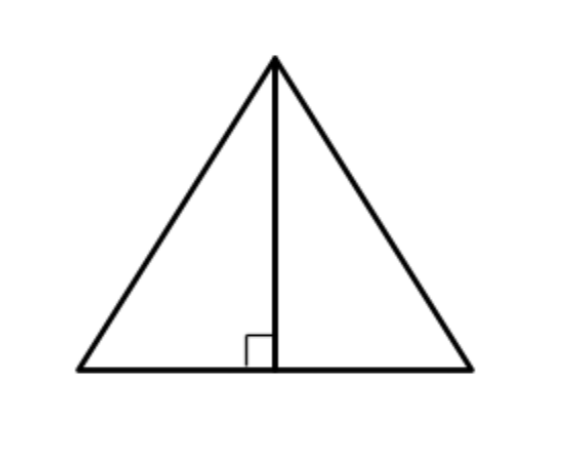
\includegraphics[width=0.4\linewidth]{Geometry/Content/18.png}
	
}

Пусть в треугольнике $ABC$ $AC = BC = 35$, $AB = 42$. Проведем высоту $CD$, которая является и медианой. Тогда $BD = \linebreak =\frac{AB}{2} = 21$. Треугольник  $BCD$ - прямоугольный, по теореме Пифагора $CD = \sqrt{BC^2 - BD^2} = \sqrt{35^2 - 21^2} = 28.$

Тогда $S_{\Delta ABC} = \frac{AB \cdot CD}{2} = BD \cdot CD = 21 \cdot 28 = 588.$ \newline \null \hspace*{\fill} Ответ: 588.

\textbf{1836-1838} - аналогичные задачи.

\textbf{1839.}  Выразим площадь треугольника через боковые стороны, равные $a$, и угол между ними $\alpha = 30^\circ$:
\[
S = \frac{a^2 \sin{\alpha}}{2} = \frac{a^2}{4}.\; Отсюда \;a = 2\sqrt{S} = 2\sqrt{529} = 46
\]. \null \hspace*{\fill} Ответ: 46.

\textbf{1840-1846} - аналогичные задачи.